%!TEX root = ../my_thesis.tex
\section{The Cabibbo-Kobayashi-Maskawa matrix}
\label{sec:ckm}

The Lagrangian density describing the weak interactions between quarks and $W^\pm$ (\emph{charged current interaction}) can be written as
\begin{equation}
	\label{eq:Lcc}
	\mathcal L_{cc} = \frac{g}{\sqrt{2}} \left( \begin{array}{ccc} \bar u & \bar c & \bar t \end{array} \right) V_{\rm CKM} \gamma^\mu \frac{\left(1-\gamma^5\right)}{2} \left( \begin{array}{c} d \\ s \\ b \end{array} \right) W^+_{\mu} + h.c.,
\end{equation}
where $g$ is a coupling constant, $\gamma^\mu$ are Dirac matrices and $V_{\rm CKM}$, known as the Cabibbo-Kobayashi-Maskawa (CKM) matrix \cite{PRL-10-1963-531,PTP-49-1973-652}, 
couples the \emph{flavour} eigenstates $d$, $s$ and $b$ to the \emph{mass} (or \emph{physical}) eigenstates $d'$, $s'$ and $b'$:
\begin{equation}
	V_{\rm CKM} = \left( \begin{array}{ccc} V_{ud} & V_{us} & V_{ub} \\ V_{cd} & V_{cs} & V_{cb} \\ V_{td} & V_{ts} & V_{tb} \end{array} \right).  
\end{equation}
The CKM matrix is unitary ($V_{\rm CKM}^\dagger V_{\rm CKM}\equiv 1$), so it can be written in terms of four independent parameters, namely three angles and a \emph{complex phase} $\delta$. 
The latter is the source of all \emph{CP-violating} phenomena in the SM, i.e. asymmetries between particles and antiparticles; in fact, the \emph{complexity} of $V_{\rm CKM}$
implies that the SM Lagrangian density is non \CP-invariant, in agreement with the experimentally observed \CP~violation.

A first, standard parameterisation of the CKM matrix \cite{PRL-53-1984-53} gives
\begin{equation}
	V_{\rm CKM} = \left( \begin{array}{ccc} c_{12}c_{13} & s_{12}c_{13} & s_{13}e^{-i\delta} \\ 
								-s_{12}c_{23}-c_{12}s_{23}s_{13}e^{i\delta} &  c_{12}c_{23}-s_{12}s_{23}s_{13}e^{i\delta} & s_{23}c_{13} \\
								s_{12}s_{23}-c_{12}c_{23}s_{13}e^{i\delta} &  -c_{12}s_{23}-s_{12}c_{23}s_{13}e^{i\delta} & c_{23}c_{13} \end{array} \right),
\end{equation}
where $s_{ij}=\sin\theta_{ij}$ and $c_{ij}=\cos\theta_{ij}$.

Another, useful parameterisation is given by \emph{Wolfenstein} \cite{PRL-51-1983-1945} and points out the order of magnitude of each matrix element. By defining the quantities $\lambda$, $A$, $\rho$ and $\eta$ with
\begin{align}
	s_{12} &= \lambda = \frac{|V_{us}|}{\sqrt{|V_{ud}|^2+|V_{us}|^2}}, & s_{23} &= A\lambda^2=A\left|\frac{V_{cb}}{V_{us}}\right|, \\
	s_{13}e^{i\delta} &= V^{*}_{ub} = A\lambda^3(\rho+i\eta), 
\end{align}
the $V_{\rm CKM}$ matrix can be rewritten as a series expansion in powers of $\lambda$, given that $\lambda$ is a small number:
\begin{equation}
	\label{eq:ckm}
	V_{\rm CKM} = \left( \begin{array}{ccc} 1-\lambda^2/2 & \lambda & A\lambda^3(\rho-i\eta) \\ 
									-\lambda & 1-\lambda^2/2 & A\lambda^2 \\
									A\lambda^3(1-\rho-i\eta) & -A\lambda^2 & 1 \end{array} \right) + \mathcal O(\lambda^4).
\end{equation}
From Eq.~\ref{eq:ckm}, one can see that quark transitions within the same family (\eg $u\to d$) are more probable, whereas transitions between different families (\eg $b\to c$) are more suppressed. \CP~violation is a consequence of $\eta\neq0$ and $\eta\neq\pi$.

The unitarity condition $V_{\rm CKM}^\dagger V_{\rm CKM}\equiv 1$ can be rewritten in terms of six scalar equations. Two of them are particularly relevant for the $b$-hadron phenomenology:
\begin{align}
	\label{eq:ut}
	V_{ud}V_{ub}^* + V_{cd}V_{cb}^* + V_{td}V_{tb}^* &= 0, \\
	\label{eq:ut_s}
	V_{us}V_{ub}^* + V_{cs}V_{cb}^* + V_{ts}V_{tb}^* &= 0.
\end{align}
These two equations can be graphically represented as \emph{triangles} is the $(\bar\rho, \bar\eta)$ complex plane,
where $\bar\rho$ and $\bar\eta$ are defined in terms of the series expansions 
$\bar\rho=\rho(1-\lambda^2/2+\dots)$ and $\bar\eta=\eta(1-\lambda^2/2+\dots)$, respectively. 
Having introduced the following angles,
\begin{align}
	\label{eq:alpha_beta}
	\alpha &= \phi_2 = \arg\left[-\frac{V_{td}V_{tb}^*}{V_{ud}V_{ub}^*}\right], & \beta &= \phi_1 = \arg\left[-\frac{V_{cd}V_{cb}^*}{V_{td}V_{tb}^*}\right], \\
	\gamma &= \phi_3 = \arg\left[-\frac{V_{ud}V_{ub}^*}{V_{cd}V_{cb}^*}\right], & \beta_s &= \chi = \arg\left[-\frac{V_{cb}V_{cs}^*}{V_{tb}V_{ts}^*}\right],
\end{align}
the triangles given by Eqs.~\ref{eq:ut} and~\ref{eq:ut_s} can be depicted as shown in Fig.~\ref{fig:ut}. The first triangle, defined by Eq.~\ref{eq:ut}, is known as the \emph{Unitarity Triangle} (UT) and its elements can be
measured from analyses of $B^0$, $B^0_s$ and $B^{\pm}$ decays. The other triangle (Eq.~\ref{eq:ut_s}) can be studied from decays of $B^0_s$ mesons.

The amount of \CP~violation in the SM is given by the Jarlskog invariant $J$~\cite{Jarlskog:1985ht}, which satisfies
\begin{equation}
  \Im\left[V_{ij}V_{kl}V^{*}_{il}V^{*}_{kj}\right] = J \sum\limits_{m,n}\varepsilon_{ikm}\varepsilon_{jln}\,,
\end{equation}
where $\varepsilon$ denotes the fully-antisymmetric tensor. The measured value of $J$ is too small by several orders of magnitude to explain the observed matter-antimatter asymmetry in the universe, according to the baryogenesis model~\cite{Sakharov:1967dj}. So, new sources of \CP~violation not foreseen by the SM have to exist, and thus measuring the UT with the highest possible precision is crucial to constrain these new physics scenarios.

\begin{figure}[htbp]
  \begin{center}
    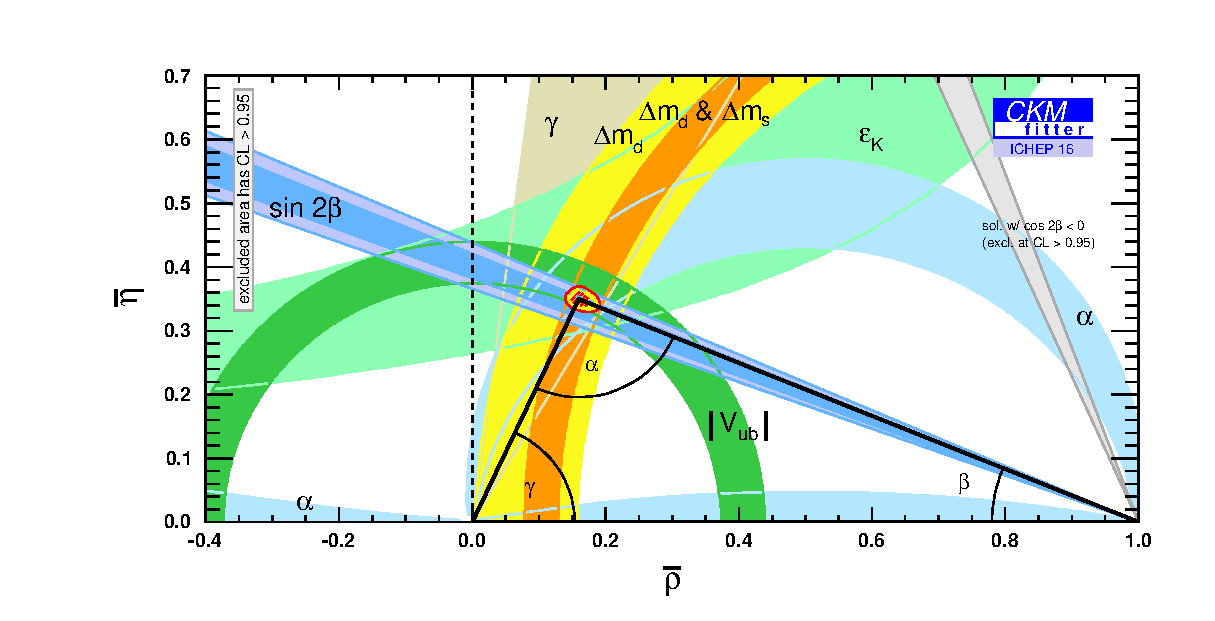
\includegraphics[width=0.9\textwidth]{02CKM/figs/ut.eps} \\
    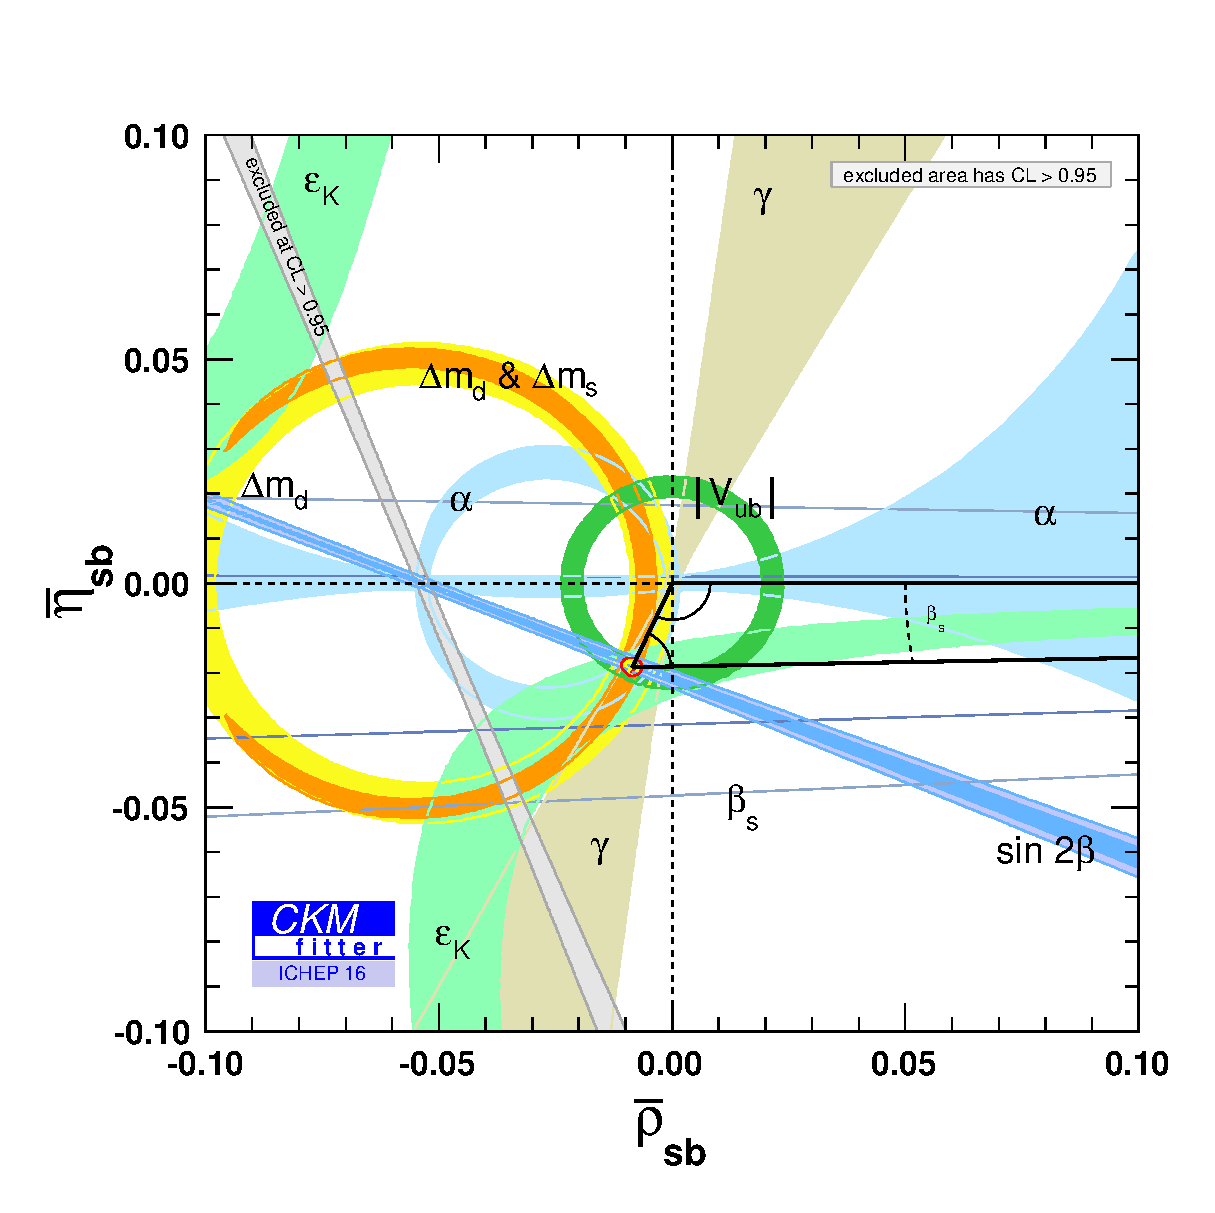
\includegraphics[width=0.9\textwidth]{02CKM/figs/ut_s.eps} \\
  \end{center}
  \vspace{-2mm}
  \caption{Graphical representation of two of the six unitarity conditions of the CKM matrix, superimposed with the current experimental constraints~\cite{CKMfitter2015}.}
  \label{fig:ut}
\end{figure}
